\documentclass[12pt]{article}
\usepackage{amsmath}
\usepackage{geometry}
\usepackage{graphicx}
\usepackage[hidelinks]{hyperref}
\usepackage[latin1]{inputenc}
\usepackage{listings}
\usepackage[dvipsnames]{xcolor}
\renewcommand{\labelitemi}{$\textendash$}
\geometry{
    a4paper,
    total={170mm,257mm},
    left=20mm,
    right=20mm,
    top=15mm,
    bottom=15mm
}

\title{CS7DS2: Week 6 Assignment}
\author{Conor McCauley - 17323203}
\date{March 16, 2022}

\begin{document}

\maketitle

\textbf{N.B.} The loss function used in this assignment is included in Appendix A.

\section*{Question (a)}

\noindent \textbf{(i)} A single Python class, \texttt{SGD}, will implement the SGD algorithm for all methods of step size calculation. The constructor takes as parameters the function being minimised, the derivative functions, the starting value of $x$, an enum specifying the choice of step size, a dictionary of hyperparameters, the batch size and the training data.

The \texttt{run\_iter\_minibatch()} method runs an iteration of mini-batch SGD:

\lstset{basicstyle=\footnotesize}
\begin{lstlisting}[language=Python]
def run_iter_minibatch(self):
    np.random.shuffle(self.T)
    N = len(self.T)
    for i in range(0, N, self.batch_size):
        if i + self.batch_size > N: continue
        sample = self.T[i:(i + self.batch_size)]
        self.iter_function(sample)
\end{lstlisting}

The method shuffles the training data, iterates over batch size-length samples of the training data (making sure not to sample outside the bounds of the array) and calls the \texttt{iter\_function()} method for that sample. This method varies depending on the choice of step size calculation but it is practically identical to the implementations provided in the previous assignment. For example, when using a constant step size \texttt{iter\_function()} would call the following method:

\lstset{basicstyle=\footnotesize}
\begin{lstlisting}[language=Python]
def __iter_constant(self, sample):
    alpha = self.params['alpha']
    for i in range(self.n):
        self.x[i] -= alpha * self.__calc_approx_derivative(i, sample)

def __calc_approx_derivative(self, i, sample):
    return sum(
        self.df[i](*self.x, *sample[j]) for j in range(self.batch_size)
    ) / self.batch_size
\end{lstlisting}

As can be seen in the above code, the only noticeable change from the previous assignment is the replacement of calls to \texttt{df} with calls to a function that uses the mini-batch sample to calculate the approximate derivative.

\vspace{3mm}
\noindent \textbf{(ii)} Figure \ref{fig:a_ii} contains a contour plot and a wireframe plot of $f(x, T)$ over the ranges $-15 \le x_0 \le 10, -15 \le x_1 \le 10$. These ranges were chosen so as to allow for a clear view of both of the function's minima while also showing its flatness when $x_1 < 0$ and steepness when $x_1 > 5$. The same training data, $T$, was used in both plots to maintain consistency:

\begin{figure}[h]
    \centering
    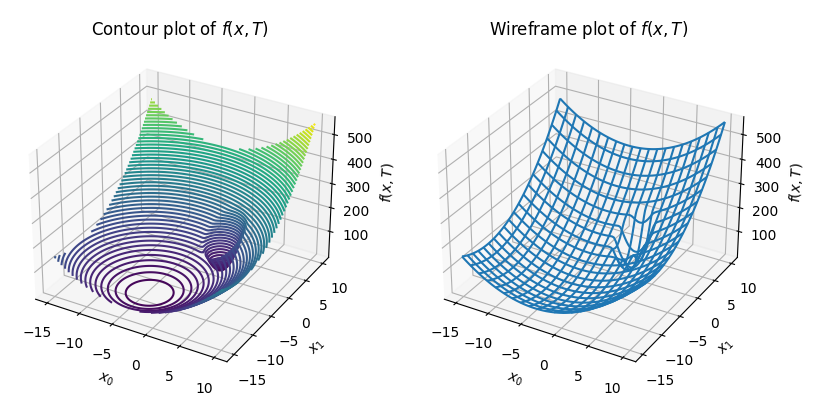
\includegraphics[scale=0.7]{figs/a/a_ii.png}
    \caption{Contour and wireframe plots of $f(x, T)$}
    \label{fig:a_ii}
\end{figure}

\vspace{3mm}
\noindent \textbf{(iii)} The part of our function that we are interested in finding the derivative of is:

$$\min(18 (z_0^2 + z_1^2), (z_0 + 10)^2 + (z_1 + 5)^2),\, z_i = x_i - w_i - 1, w \in T$$

As such, we can write our function in SymPy using four symbols, $x_0, x_1, w_0, w_1$, and differentiate it once with respect to $x_0$ and once with respect to $x_1$:

\lstset{basicstyle=\footnotesize}
\begin{lstlisting}[language=Python]
x0, x1, w0, w1 = sp.symbols('x0 x1 w0 w1', real=True)
f = sp.Min(18*(((x0-w0-1)**2)+((x1-w1-1)**2)),(((x0-w0-1)+10)**2)+(((x1-w1-1)+5)**2))
df0 = sp.diff(f, x0)
df1 = sp.diff(f, x1)
\end{lstlisting}

This code is almost identical to the SymPy code used in both previous assignments except for the inclusion of a sample of training data, $w$. The resulting derivatives are too long to include here but can be found in Appendix A.

\lstset{basicstyle=\footnotesize}
\begin{lstlisting}[language=Python]
print(df0) -> (-36*w0 + 36*x0 - 36)*Heaviside(-18*(-w0 + x0 - 1)**2 + ...
print(df1) -> (-36*w1 + 36*x1 - 36)*Heaviside(-18*(-w0 + x0 - 1)**2 + ...
\end{lstlisting}

\section*{Question (b)}

\noindent \textbf{(i)} Since running classical gradient descent (CGD) on our training data is the same as running SGD with a batch size equal to the length of our training data we can use the \texttt{SGD} class outlined in (a)(i) with the constant step size algorithm. In order to determine an appropriate step size we will experiment with a range of $\alpha \in \{0.1, 0.01, 0.001, 0.0001\}$. Running gradient descent for 100 iterations for each $\alpha$ produces the results shown in figure \ref{fig:b_i}.

\begin{figure}[h]
    \hspace*{-0.45in}
    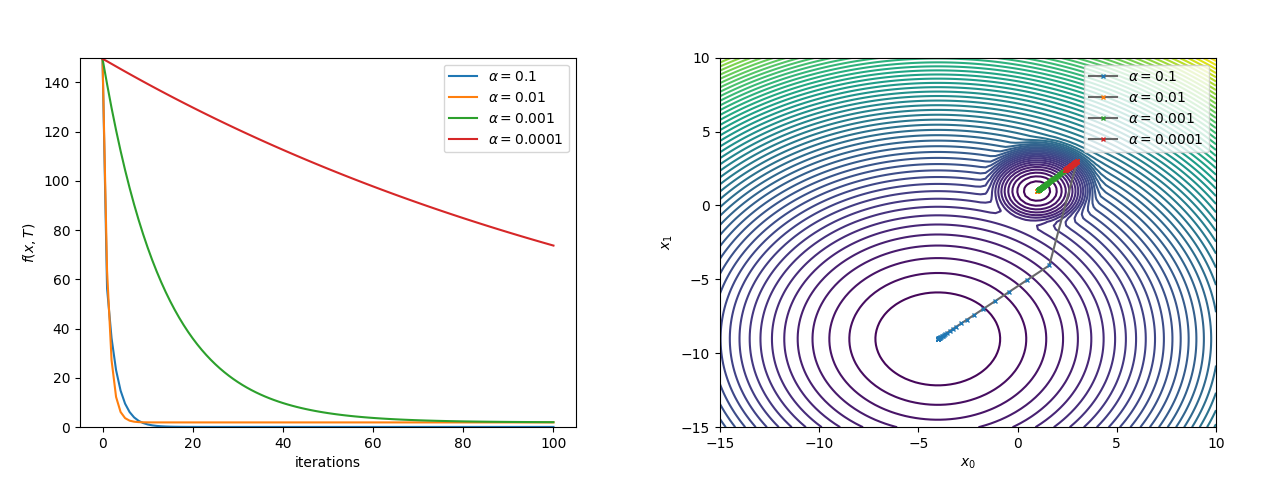
\includegraphics[scale=1.75]{figs/b/b_i.png}
    \caption{Change in $x$ and $f(x, T)$ over iterations for different $\alpha$ (CGD + constant)}
    \label{fig:b_i}
\end{figure}

It is evident from these results that $\alpha = 0.1$ is optimal as it converges on a minimum the fastest with $\alpha = 0.01$ and $\alpha = 0.001$ not converging on the global minimum and $\alpha = 0.0001$ not converging at all. The reason for this lack of convergence on the global minimum is clear from the contour plot. The noise introduced to the training data causes the minimum that all but $\alpha=0.1$ converge to be larger than zero (the function's noiseless minimum). The minimum that $\alpha=0.1$ converges to is not exactly zero either however it is a good deal closer than the other minimum. We can thus conclude that $\alpha=0.1$ is the optimal choice for our function.

\vspace{3mm}
\noindent \textbf{(ii)} Using a value of $\alpha = 0.1$ we can run five trials of our constant step size SGD each running for 10 iterations using the same set of training data. The results of each trial can be seen in figure \ref{fig:b_ii}.

\begin{figure}[h]
    \hspace*{-0.45in}
    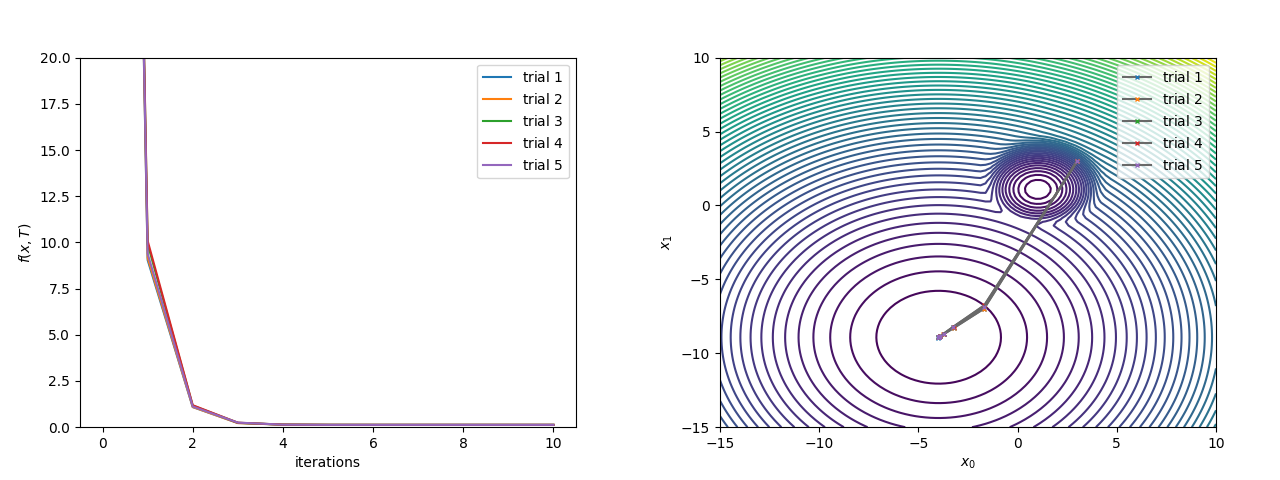
\includegraphics[scale=1.75]{figs/b/b_ii.png}
    \caption{Change in $x$ and $f(x, T)$ over iterations for $\alpha = 0.1$ (SGD + constant)}
    \label{fig:b_ii}
\end{figure}

From these results we can see that the randomness introduced during each iteration of SGD, i.e. the shuffling of the training data, has a very minor effect on the results from each of the trials. All trials converged on the minimum after around six iterations. When compared to the optimal results from (b)(i) the algorithm converged on the minimum in about half the number of iterations. Every trial also converged on the global minimum (given the noisy training data) as opposed to a local minimum.

\vspace{3mm}
\noindent \textbf{(iii)} We will use a range of batch sizes, $n$, from 1 to the size of our training data $|T|$. These values will be $n \in \{1, 3, 5, 10, 25\}$. Each trial will be run for 25 iterations. The results can be seen in figure \ref{fig:b_iii}.

\begin{figure}[h]
    \hspace*{-0.45in}
    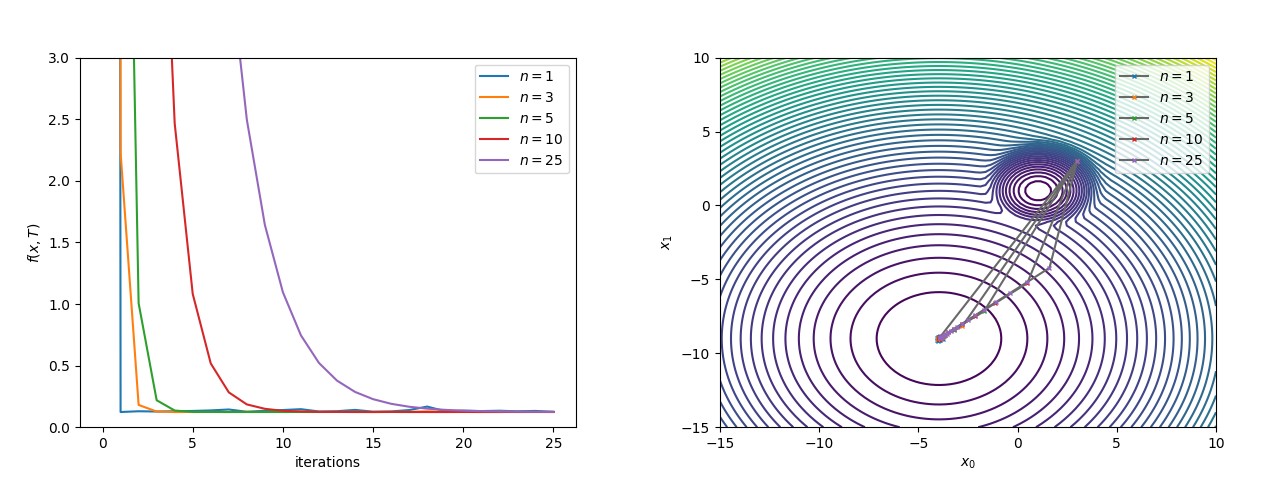
\includegraphics[scale=1.75]{figs/b/b_iii.png}
    \caption{Change in $x$ and $f(x, T)$ over iterations for different $n$ and $\alpha = 0.1$ (SGD + constant)}
    \label{fig:b_iii}
\end{figure}

All of the trials converge on the global minimum regardless of the batch size. This is probably due to $\alpha$ being large enough so as to allow the early iterations to expand $x$ far enough away from the local minimum that $x$ is initially closer to.

The number of iterations required to converge on the minimum seems to increase as $n$ is increased. However, when $n$ is very small ($n=1$) the large number of changes to $x$ that occur during each iteration, perhaps due to the noise occurring in each individual sample, seems to lead to fluctuations in $f(x, T)$ which causes poorer results. This effect occurs to a lesser degree when $n=3$ and does not appear to occur at all when $n=5$.

\vspace{3mm}
\noindent \textbf{(iv)} We will run each use the same range of values for $\alpha$ as we used in (b)(i) and run each trial for 25 iterations. The results can be seen in figure \ref{fig:b_iv}.

\begin{figure}[h]
    \hspace*{-0.45in}
    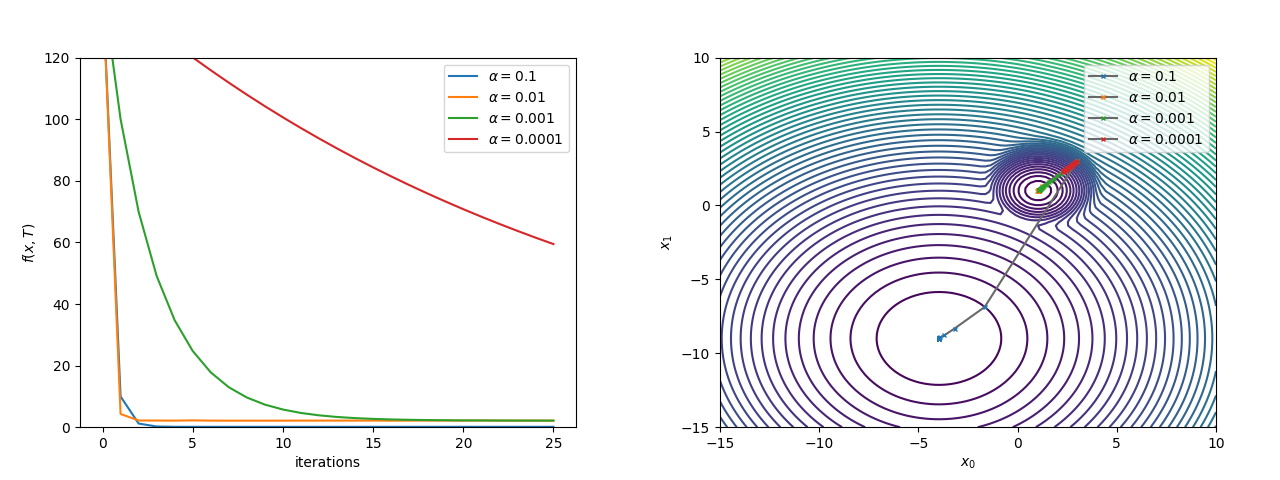
\includegraphics[scale=1.75]{figs/b/b_iv.png}
    \caption{Change in $x$ and $f(x, T)$ over iterations for different $\alpha$ (SGD + constant)}
    \label{fig:b_iv}
\end{figure}

Only the trial where $\alpha=0.1$ converges on the global minimum while the other trials all converge or begin to converge on the local minimum which is closer to the initial value of $x$. As discussed in (b)(iii), this is probably due to smaller values of $\alpha$ not expanding $x$ far enough away from its initial value in early iterations.

Due to global minimum being much flatter and consistent than the local minimum which is much steeper and confined it might be expected that the more noise is introduced to the training data the less likely the algorithm is to converge on the limited local minimum and the more likely it is to converge on the much broader global minimum. However, perhaps due to there not being `enough' noise in the training data all but one trial converges on the local minimum.

As was the case in previous trials, smaller values of $\alpha$ seem to take longer to converge. The optimal value of $\alpha$ still appears to be $0.1$ because, although the quickest convergence occurs when $\alpha = 0.01$, it does not reach the global minimum.

\section*{Question (c)}

\noindent \textbf{(i) Polyak step size:} No hyperparameters needed to be chosen for this choice of step size. SGD was run for 100 iterations for batch sizes $n \in \{1, 3, 5, 10, 25\}$ with the results from (b)(ii) being used as a baseline. The results can be seen in figure \ref{fig:c_i}.

\begin{figure}[h]
    \hspace*{-0.45in}
    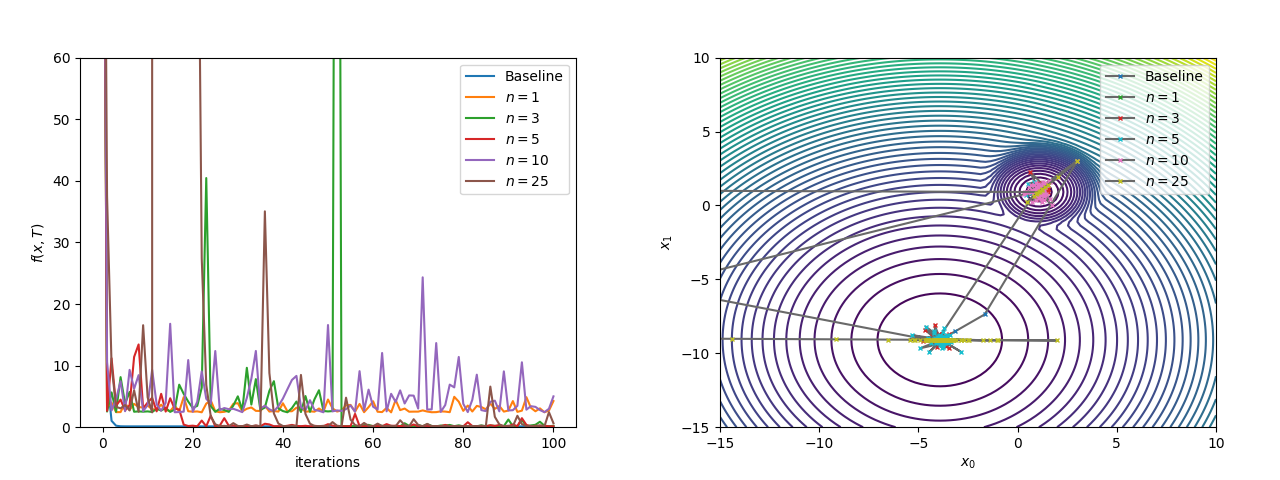
\includegraphics[scale=1.75]{figs/c/c_i.png}
    \caption{Change in $x$ and $f(x, T)$ over iterations for different $n$ (SGD + Polyak)}
    \label{fig:c_i}
\end{figure}

All of the trials appear to perform worse than the baseline. When $n=1$ and $n=10$ the functions converge on the local minimum but are relatively unstable. Each of the three cases that result in correct convergence remain somewhat unstable when compared to the baseline. A clear difference between the baseline result and the three aforementioned cases is that the latter all began converging on the local minimum before correcting themselves and converging correctly.

In this example, Polyak step size produces unstable results that do not always converge, or remain converged, on the global minimum. This is due to the step sizes during each iteration tending to be too large due to the squares of the approximate derivatives being much smaller than the value of the function itself which results in a larger than necessary step size in flatter regions of the function.

\vspace{3mm}
\noindent \textbf{(ii) RMSProp:} Hyperparameters were chosen in the ranges $\alpha_0 \in \{0.1,0.01,0.001\}$, $\beta \in \{0.25,0.9\}$ and SGD was run for 100 iterations. The results, alongside the baseline, can be seen in figure \ref{fig:c_ii_params}.

\begin{figure}[h]
    \centering
    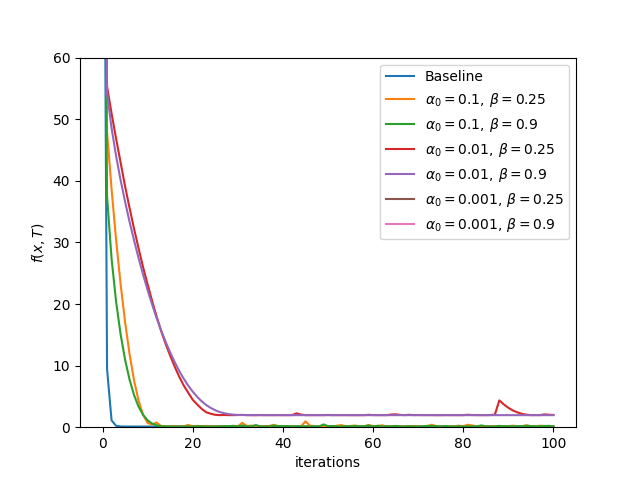
\includegraphics[scale=0.6]{figs/c/c_ii_params.png}
    \caption{Change in $f(x, T)$ over iterations for different $\alpha_0,\beta$ (SGD + RMSProp)}
    \label{fig:c_ii_params}
\end{figure}

Correct convergence occurs in the cases where $\alpha_0 = 0.1$ with the most stable results occurring when $\beta=0.9$. As such, these values will be used when varying the batch size in figure \ref{fig:c_ii}.

\begin{figure}[h]
    \hspace*{-0.45in}
    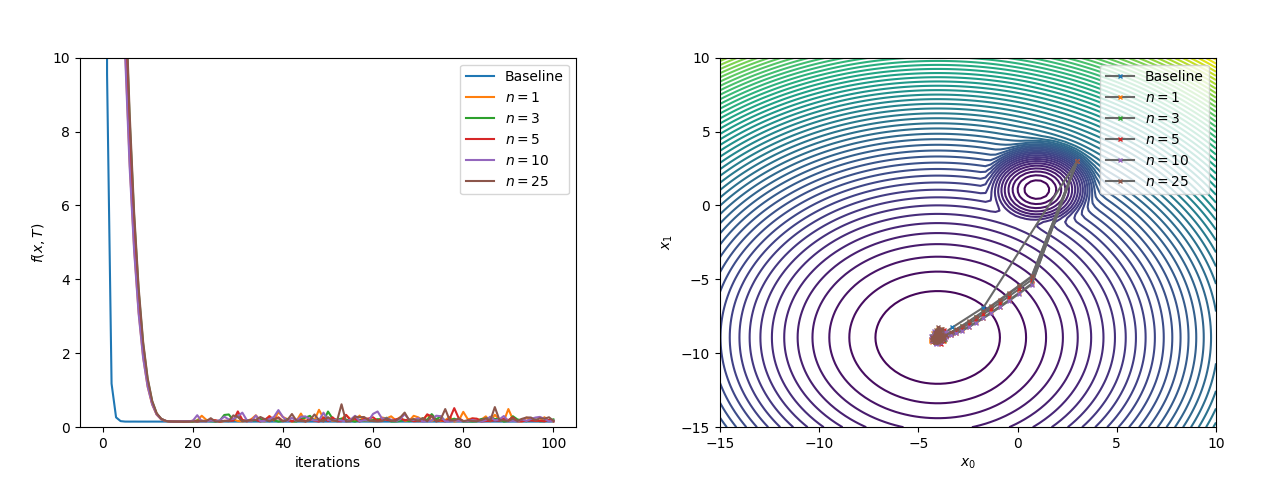
\includegraphics[scale=1.75]{figs/c/c_ii.png}
    \caption{Change in $x$ and $f(x, T)$ over iterations for different $n$ and $\alpha_0=0.1,\beta=0.9$ (SGD + RMSProp)}
    \label{fig:c_ii}
\end{figure}

All of the trials appear to perform much better than when Polyak step size was used but they still fail to outperform the baseline. Convergence on the global minimum takes about three times longer than the baseline with every trial failing to converge on a stable value. The cases where $n=3$ and $n=5$ appear to be the most stable which is consistent with the results from (b)(iii).

Unlike Polyak, flatter regions of the function do not result in an increased step size. However, the step size does not completely stabilise as it is dependent on the moving average of square gradient sums which is constantly changing during iterations.

\vspace{3mm}
\noindent \textbf{(iii) Heavy Ball:} Hyperparameters were chosen in the ranges $\alpha \in \{0.01, 0.001\}$, $\beta \in \{0.25,0.5,0.9\}$ and SGD was run for 100 iterations. The results can be seen in figure \ref{fig:c_iii_params}.

\begin{figure}[h]
    \centering
    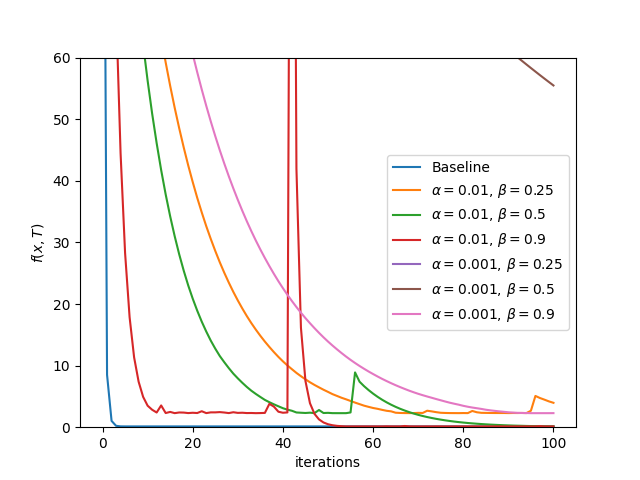
\includegraphics[scale=0.6]{figs/c/c_iii_params.png}
    \caption{Change in $f(x, T)$ over iterations for different $\alpha,\beta$ (SGD + HB)}
    \label{fig:c_iii_params}
\end{figure}

Correct convergence occurs when $\alpha=0.01$ and $\beta \in \{0.5,0.9\}$. Since convergence occurs the quickest when $\beta=0.9$ these values will be used when varying the batch size in figure \ref{fig:c_iii}.

\begin{figure}[h]
    \hspace*{-0.45in}
    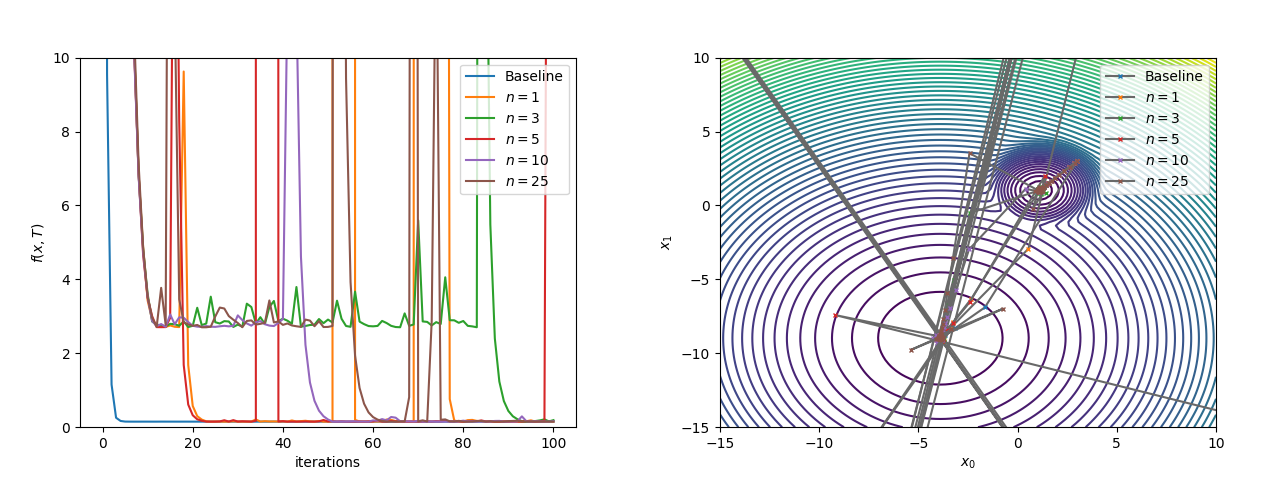
\includegraphics[scale=1.75]{figs/c/c_iii.png}
    \caption{Change in $x$ and $f(x, T)$ over iterations for different $n$ and $\alpha_0=0.01,\beta=0.9$ (SGD + HB)}
    \label{fig:c_iii}
\end{figure}

All of the trials initially begin to converge on the local minimum before eventually moving toward the global minimum. All but one of the cases appear to remain stable around the global minimum before briefly diverging away for a number of iterations before returning to the minimum. Only the case when $n=10$ appears to be stable and it is not clear if this result is reliable. It is clear that none of these results are comparable to the baseline.

Like with Polyak, the instability is due to the step size in flatter regions of the function being too large and, although this effect is reduced by $\alpha$, the repeated additions of $z\beta$ during each iteration can cause large fluctuations to occur.

\vspace{3mm}
\noindent \textbf{(iv) Adam:} Hyperparameters were chosen in the ranges $\alpha \in \{10,1,0.1\}$, $\beta_1 \in \{0.25,0.9\}$ while $\beta_2$ was kept constant at 0.999. SGD was run for 100 iterations and the results can be seen in figure \ref{fig:c_iv_params}.

\begin{figure}[h]
    \centering
    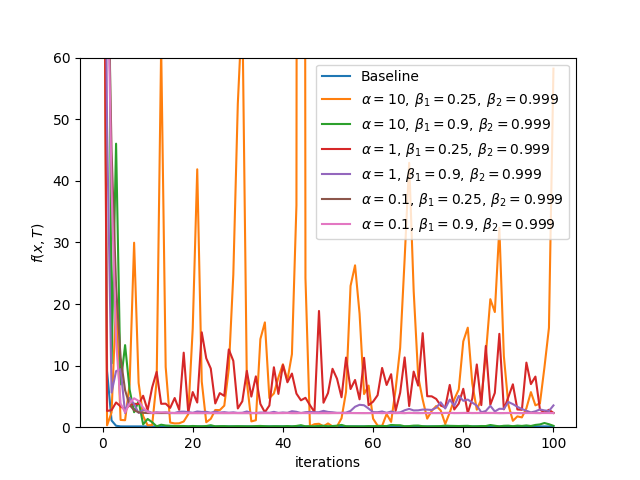
\includegraphics[scale=0.6]{figs/c/c_iv_params.png}
    \caption{Change in $f(x, T)$ over iterations for different $\alpha,\beta_1,\beta_2$ (SGD + Adam)}
    \label{fig:c_iv_params}
\end{figure}

Smaller values of $\beta_1$ appear to lead to unstable results while smaller values of $\alpha$ fail to converge on the global minimum. The only trial that managed to converge on the global minimum while also remaining stable had values of $\alpha=10$ and $\beta_1=0.9$. As such, these values will be used when varying the batch in figure \ref{fig:c_iv}.

\begin{figure}[h]
    \hspace*{-0.45in}
    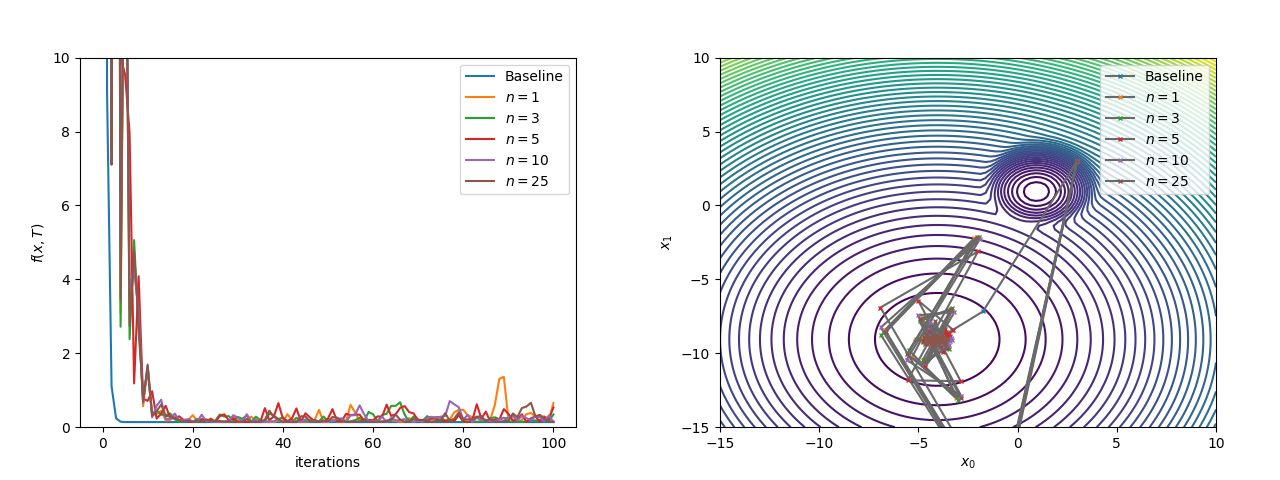
\includegraphics[scale=1.75]{figs/c/c_iv.png}
    \caption{Change in $x$ and $f(x, T)$ over iterations for different $n$ and $\alpha=10,\beta_1=0.9,\beta_2=0.999$ (SGD + Adam)}
    \label{fig:c_iv}
\end{figure}

All of the trials converge on the global minimum after around the same number of iterations but none manage to remain stable. It is difficult to tell which choice of batch size produced the best results but it appears that $n=1$ was the worst.

Like RMSProp, the step size does not stabilise due to the moving average of square gradient sums constantly changing during iterations.

\newpage
\section*{Appendix A: Code}

\lstset{basicstyle=\footnotesize,xleftmargin=0in}
\lstinputlisting[language=Python]{main.py}

\end{document}
